% Change 'digital' to 'printed' before printing
\documentclass[
  digital, %% This option enables the default options for the
           %% digital version of a document. Replace with `printed`
           %% to enable the default options for the printed version
           %% of a document.
  table,   %% Causes the coloring of tables. Replace with `notable`
           %% to restore plain tables.
  lof,     %% Prints the List of Figures. Replace with `nolof` to
           %% hide the List of Figures.
  lot,     %% Prints the List of Tables. Replace with `nolot` to
           %% hide the List of Tables.
  oneside,
  %% More options are listed in the user guide at
  %% <http://mirrors.ctan.org/macros/latex/contrib/fithesis/guide/mu/fi.pdf>.
]{fithesis3}
%% The following section sets up the locales used in the thesis.
\usepackage[resetfonts]{cmap} %% We need to load the T2A font encoding
\usepackage[main=english, slovak]{babel}

%% For non-Latin scripts, it may be necessary to load additional
%% fonts:
\usepackage{paratype}
%%
%% The following section sets up the metadata of the thesis.
\thesissetup{
    date          = 2017/5/22,
    university    = mu,
    faculty       = fi,
    type          = mgr,
    author        = Zuzana Dankovčíková,
    gender        = f,
    advisor       = Bruno Rossi PhD,
    title         = {Custom Roslyn Tool for Real-Time Static Code Analysis},
    TeXtitle      = {Custom Roslyn Tool for Real-Time Static Code Analysis},
    keywords      = {roslyn, C\#, compilers, code review, .NET compiler platform, Kentico, analyzer, code fix...},
    TeXkeywords   = {roslyn, C\#, compilers, code review, .NET compiler platform, Kentico, analyzer, code fix..., \ldots},
}
\thesislong{abstract}{
    TODO: This is the abstract ...
}
\thesislong{thanks}{
    TODO: This is the acknowledgement\dots

}

%% The following section sets up the bibliography.
\usepackage{csquotes}
\usepackage[              %% When typesetting the bibliography, the
  backend=biber,          %% `numeric` style will be used for the
  style=numeric,          %% entries and the `numeric-comp` style
  citestyle=numeric-comp, %% for the references to the entries. The
  sorting=none,           %% entries will be sorted in cite order.
  sortlocale=auto         %% For more unformation about the available
]{biblatex}               %% `style`s and `citestyles`, see:
%% <http://mirrors.ctan.org/macros/latex/contrib/biblatex/doc/biblatex.pdf>.
\addbibresource{mybib.bib} %% The bibliograpic database within
                          %% the file `example.bib` will be used.

\usepackage{makeidx}      %% The `makeidx` package contains
\makeindex                %% helper commands for index typesetting.

%% These additional packages are used within the document:
\usepackage{paralist}
\usepackage{amsmath}
\usepackage{amsthm}
\usepackage{amsfonts}
\usepackage{url}
\usepackage{menukeys}

\begin{document}
% =================================================================
% ============================= CHAPTER 1 =========================
% =================================================================
\chapter{Introduction}
TODO...

Ideas:

What is code quality, why is it important, tool that support it.. compilers, diversion ... aaaand here comes Roslyn which provides compiler as a platform.  

In~the~.NET world, the~compiler used~to~be a~black box that given the~file paths to~the~source text, produced an~executable (see Figure~\ref{fig:compiler-as-a-black-box}). In~order~to do that, compiler has to collect large amount of~information about the~code it is processing. This knowledge, however, was unavailable to~anyone but the~compiler itself and it was immediately forgotten once the~translated output was produced~\cite{roslyn-overview-github}. 

Why is this an~issue when for decades this black-boxes served us well? Programmers are increasingly becoming reliant~upon the~powerful integrated development environments (IDEs). Features like IntelliSense, intelligent rename, refactoring or~"Find all references" are key~to~developers' productivity; and~even more so in~an~enterprise-size systems. 

This gave a~rise to~number of~tools that analyze the~code for common issues and are able to~suggest a~refactoring. The problem is that that such~tool needs to~parse the~code first in~order~to be~able~to~understand and~analyze it. As a result companies need to invest fair amount of resources to duplicate the logic that the .NET compiler already possesses. Not only is it possible that the compiler and the tool may disagree on some specific piece of code, but with every new version of C\# the tool needs to be updated to handle new language features\cite{dot-net-development-using-the-compiler-api}.

With roslyn.. etc. etc. .. API for analysis.. use in companies for custom analyzers... etc. etc....
 https://github.com/dotnet/roslyn/wiki/Roslyn Overview -- motivation
Make sure to stress out that ".NET Compiler Platform" and "Roslyn" names will be used interchangably as it is in Roslyn Succinctly on page 11.
% =================================================================
% ============================= CHAPTER 2 =========================
% =================================================================
  \chapter{Code Quality and Static Code Analysis}
TODO

% =================================================================
% ============================= CHAPTER 3 =========================
% =================================================================
  \chapter{.NET Compiler Platform}
As~per~\cite{dragon-book}, compiler is a~program that can read a~program in a~\textit{source} language and~translate it into a~semantically equivalent program in~\textit{target} language while reporting any errors detected in~the~translation process. 

In~the~.NET world, the~compiler used~to~be a~black box that given the~file paths to~the~source text, produced an~executable (see Figure~\ref{fig:compiler-as-a-black-box}). This perception was changed in~2015 when Microsoft introduced the .NET Compiler Platform (commonly referred to as "Project Roslyn").  

\begin{figure}[h!]
		\centering
			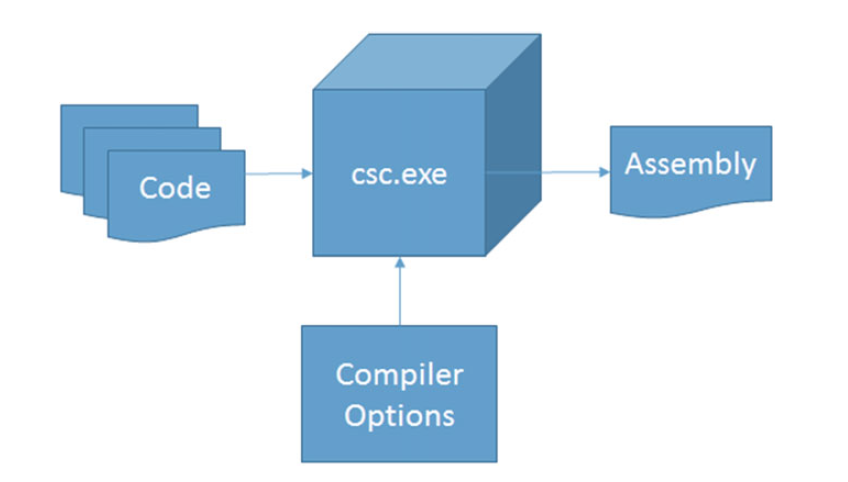
\includegraphics[scale=0.35]{img/compiler-as-a-black-box}
		\caption{Compiler as a black box~\cite{dot-net-development-using-the-compiler-api}}
		\label{fig:compiler-as-a-black-box}
\end{figure}

Not only have been compilers for both VisualBasic and C\# rewritten into entirely managed code, they also expose the internals of the compiler pipeline via a public .NET API~\footnote{Application Programming Interface}. This makes them a platform (also known as \textit{compiler-as-as-service}) with rich code analysis APIs that can be leveraged by developers to perform analysis, code generation or dynamic compilation in their own programs~\cite{roslyn-succinctly}. Those can be later easily integrated into VisualStudio all without the hard work of duplicating compilers' parsing logic.

This chapter will take a look at how the Roslyn API layers are structured, how the original source code is represented by the compiler and how developers can build tools upon the compiler's API. Lastly it will provide a short overview and evaluation of other tools that were used before Roslyn or have emerged thanks to .NET Compiler Platform.

Note that although Roslyn provides equivalent APIs for both VisualBasic and C\#, this thesis will only focus on the C\# part, since only that one is relevant for the practical part of the thesis.  
  
  \section{The Compiler Pipeline}
Roslyn compilers expose an API layer that mirrors the traditional compiler pipeline (see \ref{fig:roslyn-compiler-pipeline}). Instead of a single process of generating the target program, each compilation step is treated as a separate component~\cite{roslyn-overview}:
\begin{itemize}
  \item \textbf{Parse phase} consists of \textit{lexical analysis} (\textit{scanner}) and \textit{syntactic analysis} (\textit{parser}). First, the lexical analyzer processes the stream of characters from the source program and groups them into a meaningful sequences called \textit{lexemes}. Those are subsequently processed by the \textit{syntax analyzer} that creates a tree-like structure of tokens based on the language grammar~\cite{dragon-book}.
  \item \textbf{Symbols and metadata phsase} where named symbols are generated based on the declarations from the source and imported metadata.
  \item \textbf{Bind phase} in which the identifiers from the source code are matched to their respective symbols.
  \item \textbf{Emit phase} where all the gathered information is used to emmit an assembly.
\end{itemize}

\begin{figure}[h!]
		\centering
			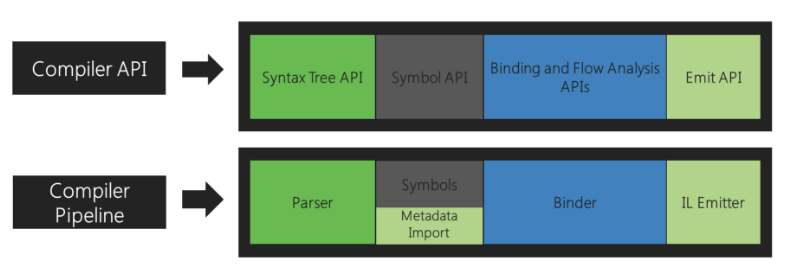
\includegraphics[scale=0.5]{img/roslyn-compiler-pipeline}
		\caption{Compiler pipeline~\cite{roslyn-overview}}
		\label{fig:roslyn-compiler-pipeline}
\end{figure}

The .NET Compiler Platform creates an object model containing information obtained by each phase and exposes it through the API in form of .NET objects. These object are also used internally by VisualStudio~\footnote{The new generation of VisualStuio leveraging from the Roslyn compiler are called vNext and first one was VS 2015.} to support basic IDE functionality. For instance \textbf{syntax tree}, that is the result of the parse phase, is used to support formatting and colorizing the code in the editor. The result of the second phase -- \textbf{hierarchical symbol table}, is the basis for "Object browser" and "Navigate to" functionality. Binding phase is represented as an \textbf{object model that exposes the result of the semantic analysis} and is utilized in "Find all references" or "Go to definition". Finally, the Emit phase produces the Intermediate Language (IL) byte codes and is also used for "Edit and Continue" feature~\cite{roslyn-overview}.

  \section{The .NET Compiler Platform's Architecture}
The Roslyn's architecture consists of two main layers (Compiler and Workspaces) and one secondary layer (Features), as seen on Figure~\ref{fig:roslyn-compiler-architecture}.

\begin{figure}[h!]
		\centering
			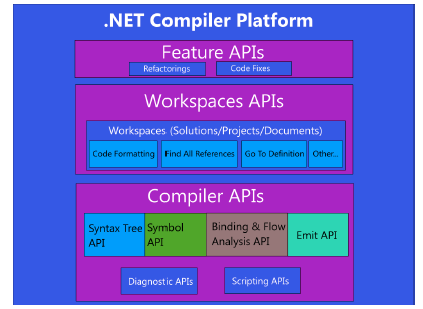
\includegraphics[scale=0.6]{img/roslyn-compiler-architecture}
		\caption{Compiler pipeline~\cite{roslyn-succincly}}
		\label{fig:roslyn-compiler-architecture}
\end{figure}

One of the key concepts of .NET Compiler Platform is immutability. The compiler exposes hundreds of types that represent all information about source code from \texttt{Project} and \texttt{Document} to \texttt{SyntaxTrees} with almost all of those types being immutable. This means, that once created, the object cannot change. In order to alter it in any way, new instance must be created, either manually, or from an existing instance by applying one of many \texttt{With...()} methods that the API provides.

The Immutability enables the compiler to perform parallel work without need to create duplicate objects or apply any locks on them. The concept is useful for the command line compiler but it is considered extremely important for IDEs where it enables one document to be analyzed by multiple analyzers in parallel.

  \subsection{The Compiler APIs}
As discussed in the previous section, the Compiler APIs offer an object model representing the results of syntactic and semantic analysis produced by the respective phases of the compiler pipeline. Moreover, it also includes an immutable snapshot of a single compiler invocation, along with assembly references, compiler options, and source files. This layer is completely agnostic of any Visual Studio components and as such can be used in stand-alone applications as well. There are two separate, though very similar, APIs for Visual Basic and C\#, each providing functionality tailored for specific language nuances.

  \subsubsection{Diagnostic APIs}
Apart from parsing code and producing an assembly, the compiler is also capable of raising diagnostics, covering everything from syntax to semantics, and report them as errors, warnings or information messages~\cite{roslyn-succinctly}. This is achieved through the compilers' Diagnostics APIs that allow developers to effectively plug-in to compiler pipeline, analyze the source code using the exposed object models, and surface custom diagnostics along with those defined by compiler itself. These APIs are integrated to both MSBuild~\footnote{Does this needs an explanation??} and Visual Studio~\footnote{Visual Studio 2015 and newer.} providing seamless developer experience. The practical part of this thesis hugely relies on Diagnostic APIs to provide custom diagnostics, the details will be discussed in the \pageref{chap:custom-roslyn-analyzers}.

  \subsubsection{Scripting APIs}
As a part of the compiler layer, Microsoft team has introduced new Scripting APIs that can be used for executing code snippets. This APIs were not shipped with .NET Compiler Platform 1.0 and are part of v2.0.0 Release Candidate 3\footnote{As per https://github.com/dotnet/roslyn/wiki/Scripting-API-Samples [26-02-2017].}.

  \subsection{Workspaces APIs}
Workspace represents a collections of solutions, projects and documents. It is a starting point for performing code analysis and refactorings over entire solutions. It provides a single object model containing information about the projects in a solution and their respective documents; exposes all configuration options, assembly and inter-project dependencies, and provides access to syntax trees and semantic models. 

Although it is possible to use the Workspace outside of any host environment, the most common use case is an IDE providing an instance of Workspace that corresponds to the open solution. Since the instances of Solution are immutable, the host environment must react to every event (such as user key stroke) with an update of the \texttt{CurrentSolution} property of the Workspace. This cycle is illustrated in Figure~\ref{fig:host-environment-and-workspaces}.

\begin{figure}[h!]
		\centering
			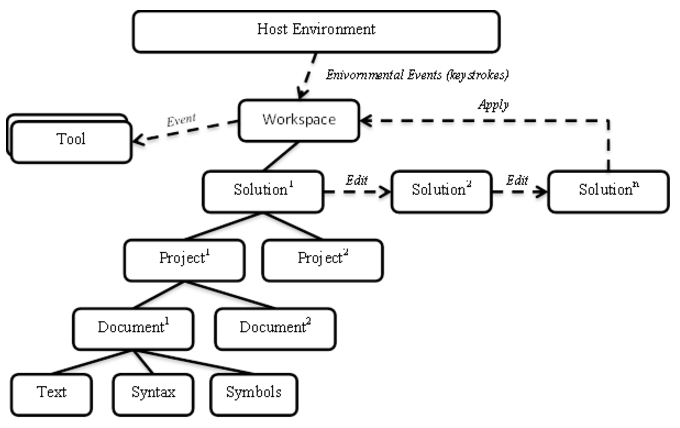
\includegraphics[scale=0.6]{img/host-environment-and-workspaces}
		\caption{Compiler pipeline~\cite{roslyn-overview}}
		\label{fig:host-environment-and-workspaces}
\end{figure}
  
  \subsection{Feature APIs}
This layer relies on both Compiler and Workspaces layers and is designed to provide API for offering code fixes and refactorings. This layer was also utilized while working on the practical part of this thesis.
  

  
  \section{Syntax}

  \section{Semantics}

  \section{Analysers and Code Refactorings}
%  - how to perform static code analysis with Roslyn
%    - writing anlyzers and code fixes / code refactorings  
  
  \section{Other Tools}
  %3. Other tools for code analysis available for C#
%  - new DotNetAnalyzers available thanks to Roslyn
%  - Resharper,
%  - FxCop
%  - StyleCop

% =================================================================
% ============================= CHAPTER 4 =========================
% =================================================================
Current situation \& motivation

% =================================================================
% ============================= CHAPTER 4 =========================
% =================================================================
\chapter{Custom Roslyn Analyzers}
\label{chap:custom-roslyn-analyzers}

% =================================================================
% =============================== STUFF ===========================
% =================================================================
	% From template
	\makeatletter\thesis@blocks@clear\makeatother
	\phantomsection %% Print the index and insert it into the
	\addcontentsline{toc}{chapter}{\indexname} %% table of contents.

	\printindex
    
% =================================================================
% =========================== BIBLIOGRAPHY ========================
% =================================================================
    \printbibliography

% =================================================================
% ============================ APPENDICES =========================
% =================================================================    
	\appendix %% Start the appendices.
  \chapter{Upgrades and Versioning}
TODO...

\end{document}
